%************************************************
\chapter{Prototypische Implementierung}\label{kap:prototyp}
%************************************************

Beschreibung der Architektur \\

\section{Funktioinstest}

\begin{figure}[bth]
        \myfloatalign
        {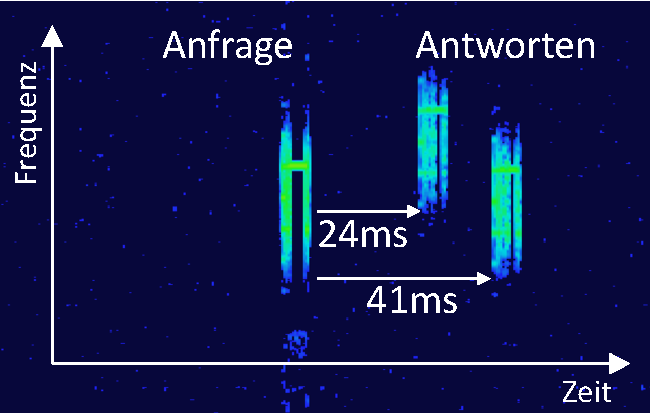
\includegraphics[width=0.6\linewidth]{gfx/Vers_01_Spac}} 
        \caption[Spektrumanalyzer]{ToDo}\label{fig:spac_2antworten}
\end{figure}

\begin{figure}[bth]
        \myfloatalign
        \subfloat[Terminal: Daten zur Übermittlung durch den \acs{ap}]
        {\label{fig:terminal-TX}%
         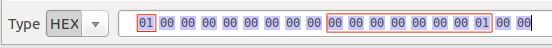
\includegraphics[width=0.8\linewidth]{gfx/ScS_Terminal_Send_markiert}} \\
        \subfloat[Terminal: Empfangene Daten am \acs{ap}]
        {\label{fig:terminal-RX}%
        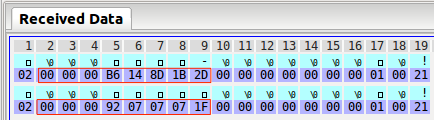
\includegraphics[width=0.8\linewidth]{gfx/ScS_Terminal_Rec_1x2Boxen_Vers_001_markiert}} 
        \caption[Terminal TX RX]{Ausschnitt aus dem Terminalprogramm \emph{hterm}. a) Sendezeile mit Bytes einer PAGE-Nachricht b) Empfagsbereich mit zwei QUANTITY-Nachrichten}\label{fig:terminal}
\end{figure}

\begin{figure}[bth]
        \myfloatalign
        {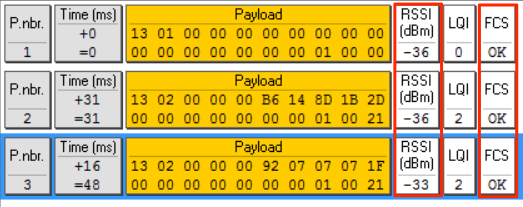
\includegraphics[width=0.8\linewidth]{gfx/ScS_Sniffer_AP_2Boxen_Vers_001_markiert}} 
        \caption[Sniffer]{Ausgabe der mitgeschnittenen Kommunikation in der \emph{Packet Sniffer} Software. Die Zusatzinformationen zu Signalstärke und Bitfehlern sind rot markiert.}\label{fig:sniffer}
\end{figure}

\begin{figure}[bth]
        \myfloatalign
        {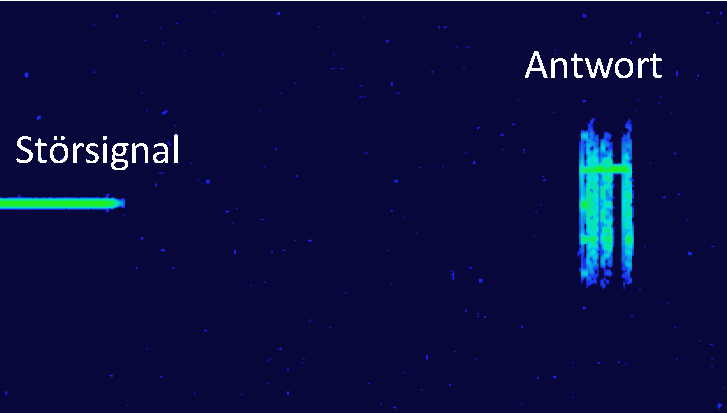
\includegraphics[width=0.6\linewidth]{gfx/Stoerer_Spac}} 
        \caption[Störsender]{Zeitlicher Verlauf der Kanalaktivität mit schmalbandigem Störsignal. Nachdem der Kanal frei ist, erscheint das Paket.}\label{fig:spac_stoerer}
\end{figure}

\section{Messungen}

\begin{figure}[bth]
        \myfloatalign
        \subfloat[Detaillierte Darstellung der Leistungsaufnahme über die Zeit bei $25ms$ Backoff]
        {\label{fig:power_csma_25zoom}%
         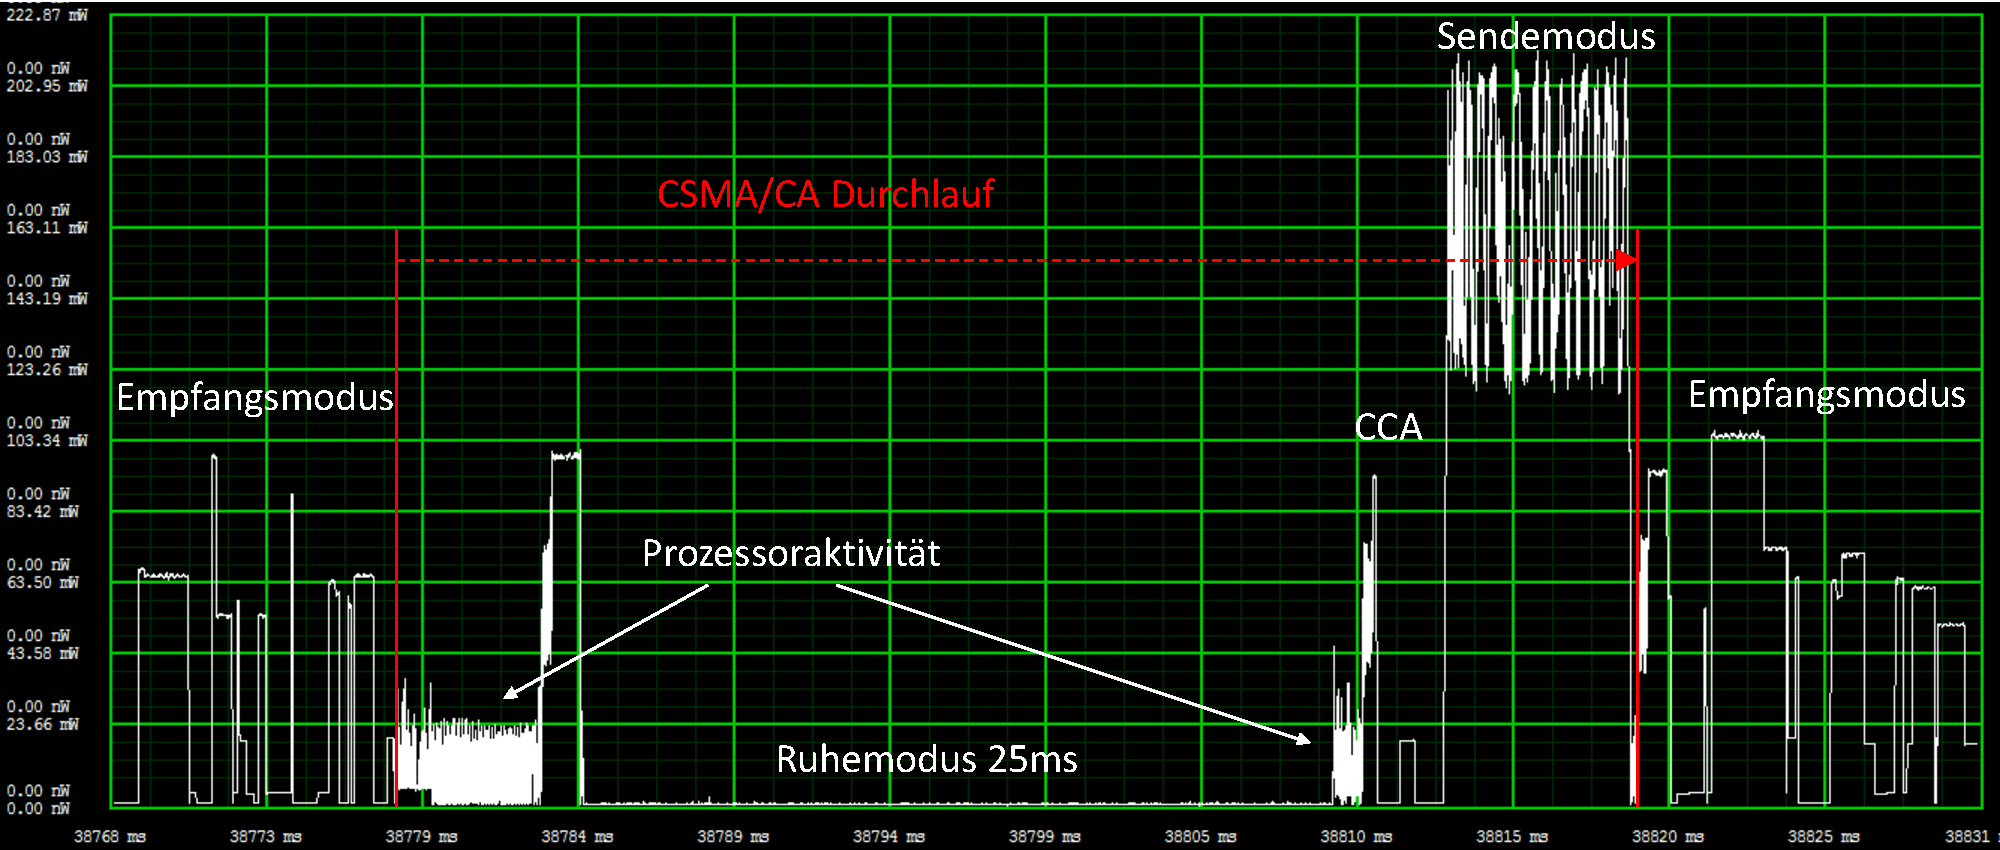
\includegraphics[width=1\linewidth]{gfx/Uebersicht_25_zoom_BO}} \\
        \subfloat[Leistungsaufnahme über die Zeit bei $34ms$ Backoff]
        {\label{fig:power_csma_34}%
        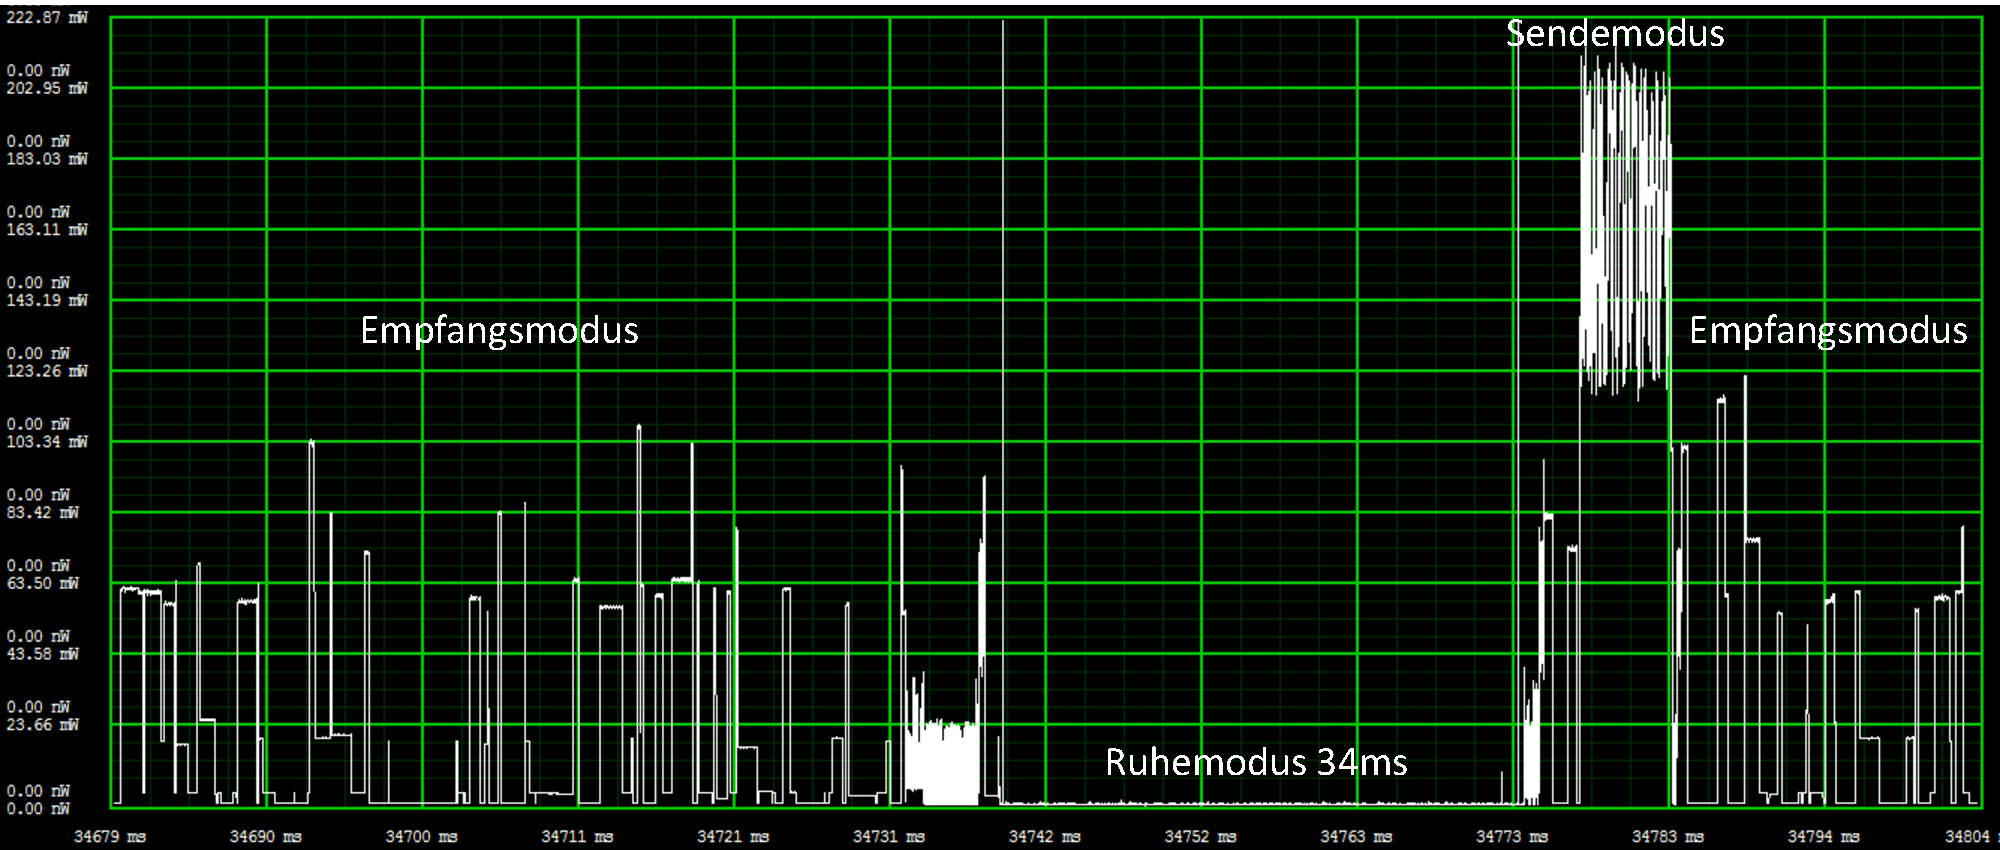
\includegraphics[width=1\linewidth]{gfx/Uebersicht_34_BO}} \\
        \subfloat[Leistungsaufnahme über die Zeit bei $101ms$ Backoff]
        {\label{fig:fig:power_csma_101}%
        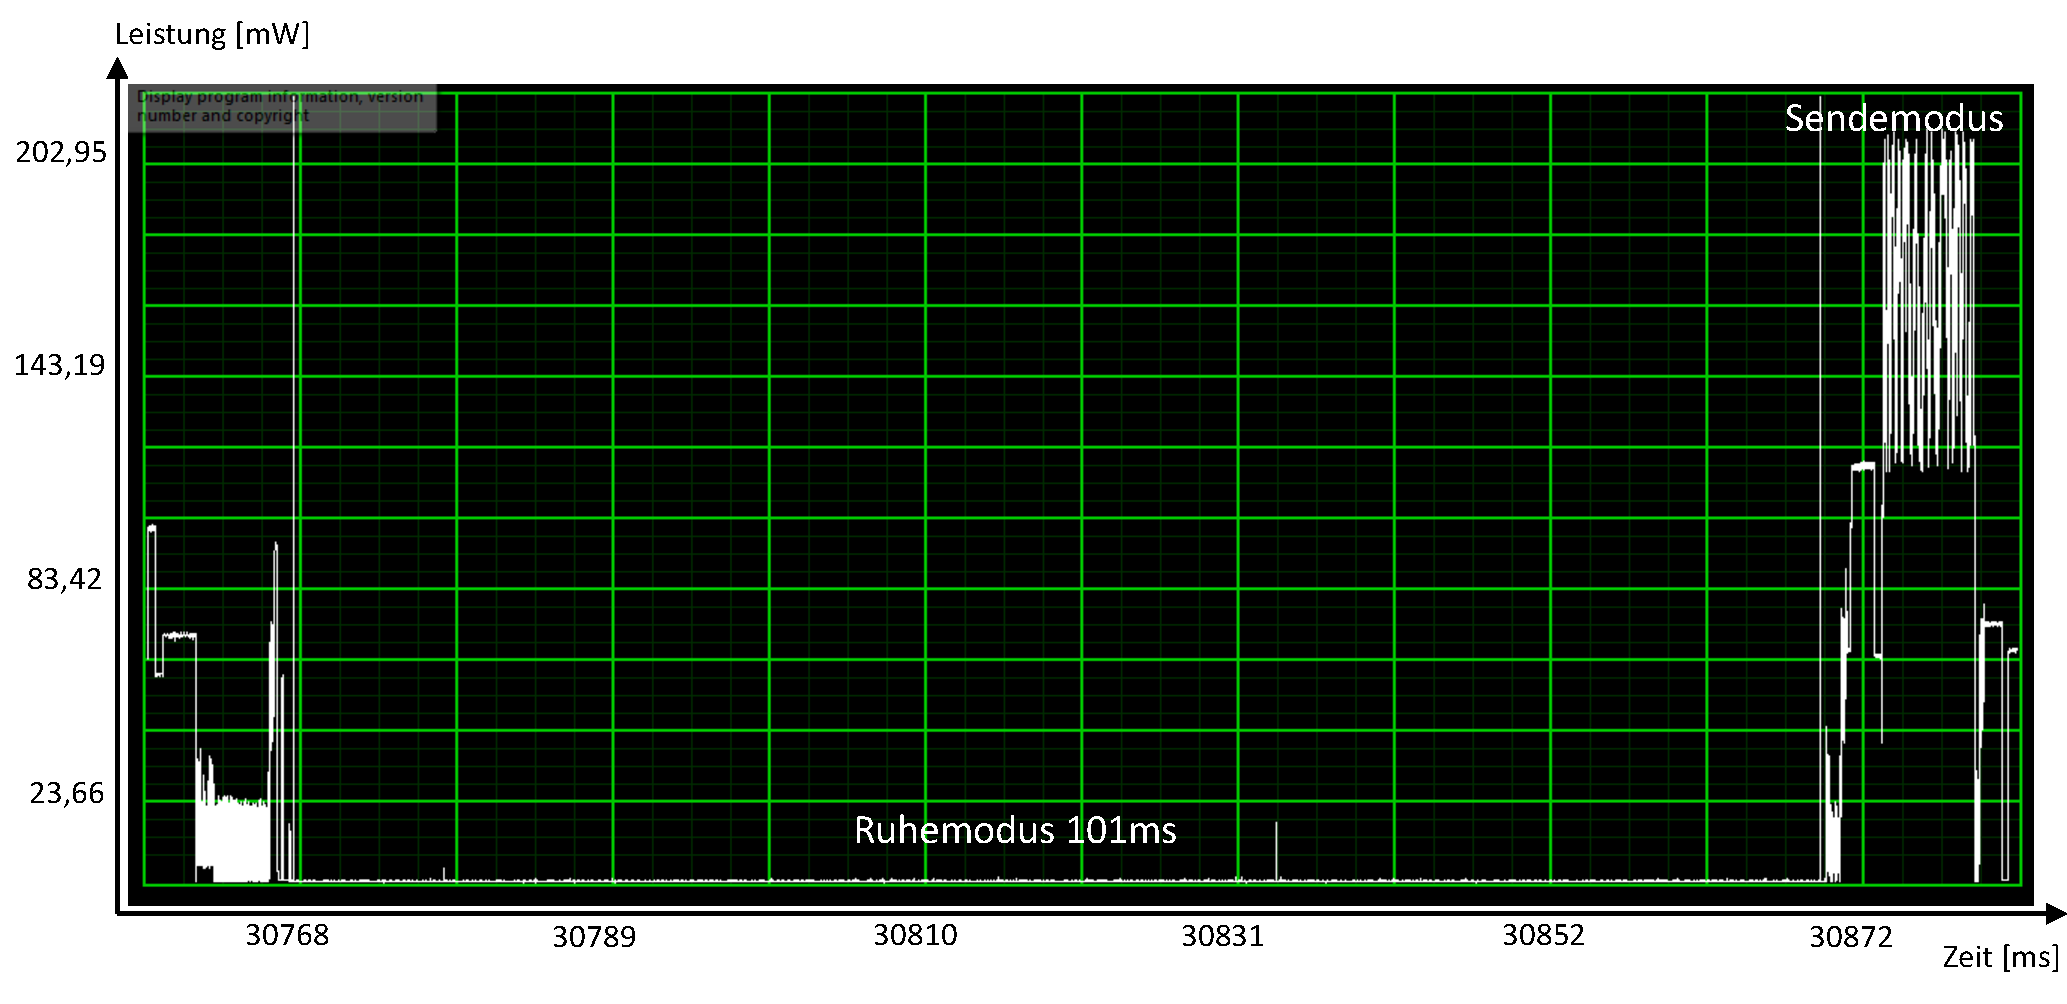
\includegraphics[width=1\linewidth]{gfx/Uebersicht_101_BO}} 
        \caption[Energiemessung CSMA/CA]{Drei Messungen des \emph{PowerScale} Systems zum Energieverbrauch des cc1200 Funkchips während des \acs{csma} Algorithmus}\label{fig:power_csma}
\end{figure}

\begin{figure}[bth]
        \myfloatalign
        {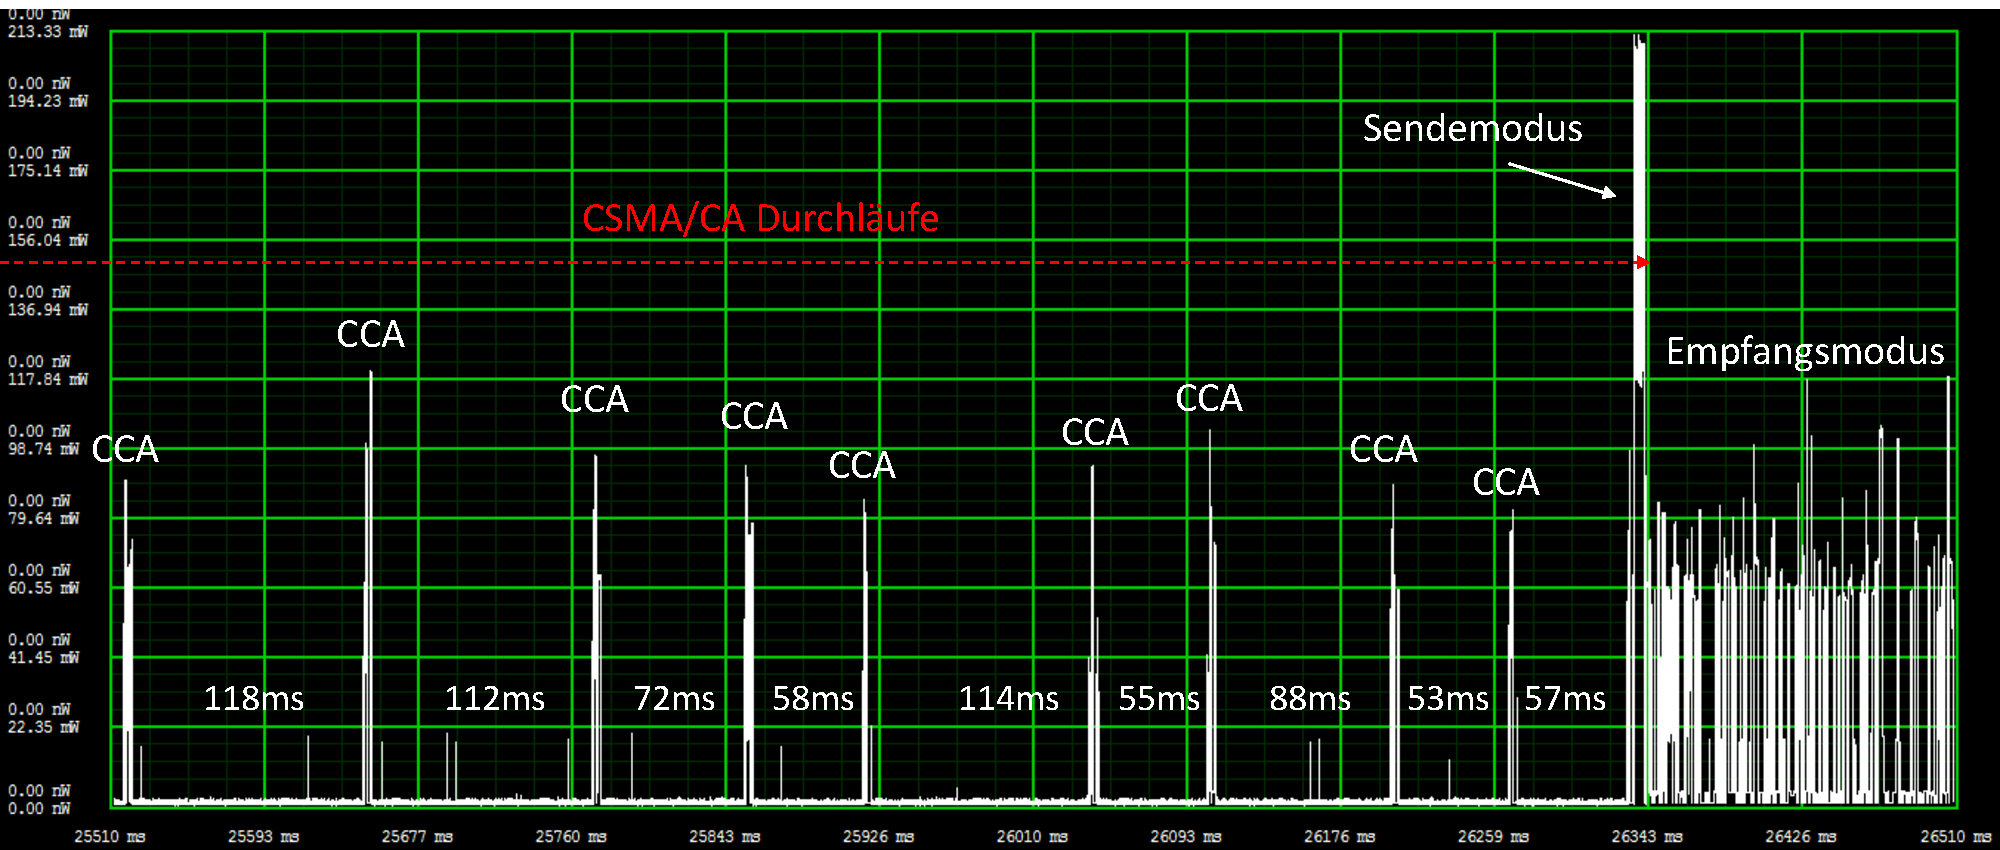
\includegraphics[width=1\linewidth]{gfx/CCA_Stoerer_Power}} 
        \caption[Energiemessung CCA]{Analyse des Energieverbrauchs während des \acs{cca}. Da der Kanal durch ein Störsignal belegt ist, werden während des \acs{csma} Algorithmus wiederholt \acsp{cca} durchgeführt.}\label{fig:power_cca}
\end{figure}

\begin{figure}[bth]
        \myfloatalign
        \subfloat[]
        {\label{fig:diag_cca_dauer_leistung}%
         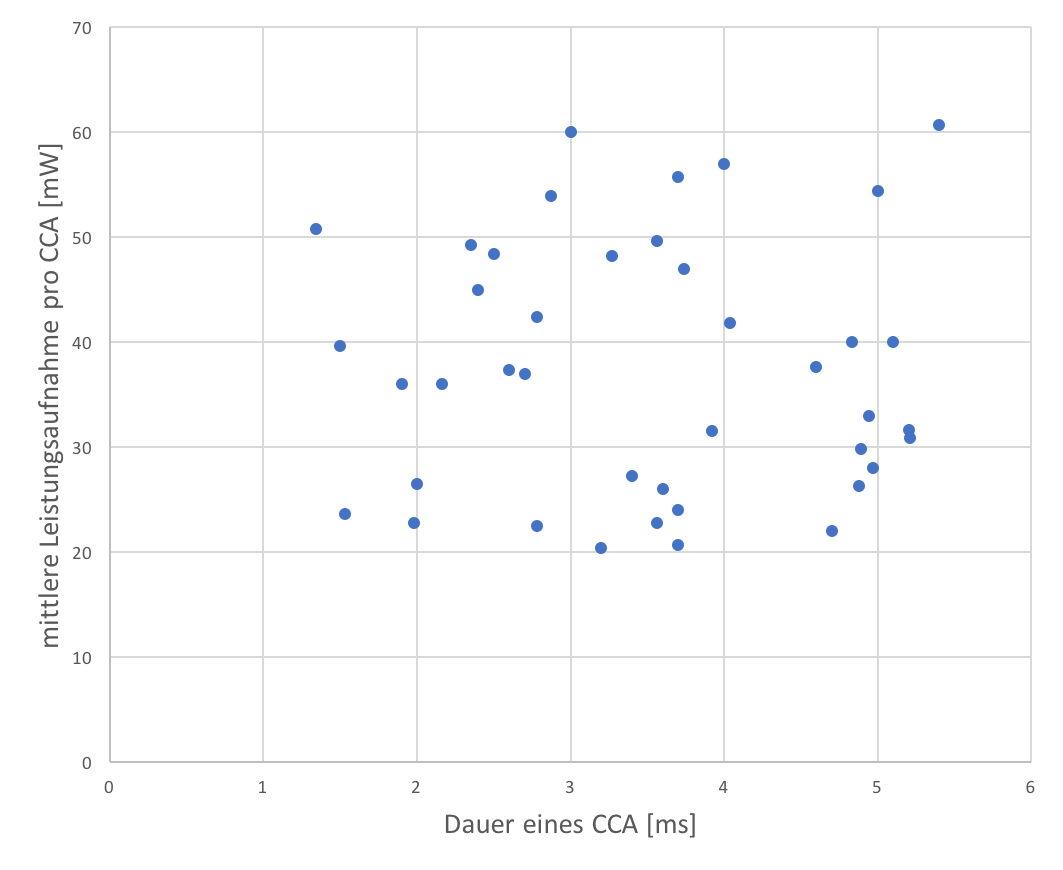
\includegraphics[width=0.75\linewidth]{gfx/Diag_CCA_Leistung_Dauer}} 
        \subfloat[]
        {\label{fig:diag_cca_energie}%
        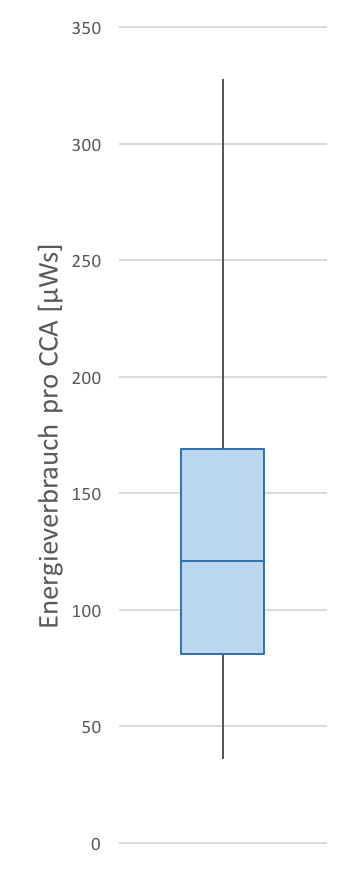
\includegraphics[width=0.25\linewidth]{gfx/Diag_CCA_Boxplot_Energie}} 
        \caption[Energiemessung CCA]{Analyse des Energieverbrauchs: a) Punktdiagramm von 40 \acs{cca} Messungen. Ein Messpaar besteht aus der Dauer und der mittleren Leistungsaufnahme b) Boxplot zum resultierenden Energieverbrauch von 40 \acsp{cca}.}\label{fig:diag_cca_dauer_leistung}
\end{figure}

\begin{figure}[bth]
        \myfloatalign
        {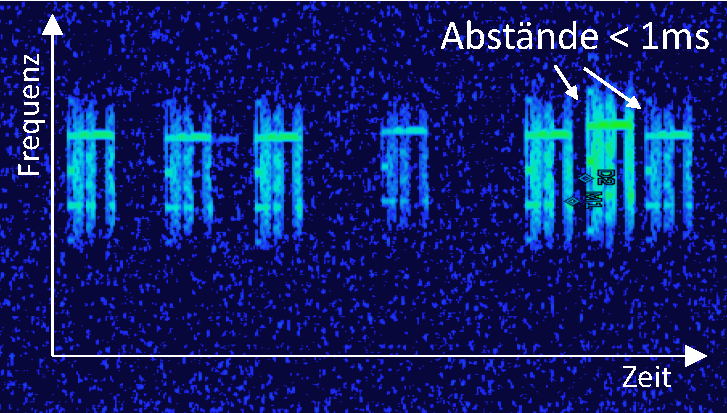
\includegraphics[width=0.6\linewidth]{gfx/Problem_Verarbeitung}} 
        \caption[Pakete mit kurzen Abstand]{Am \emph{Spectrum Analyzer} sind sieben Pakete zu sehen. Die Zwischenankunftszeit der letzten beiden Pakete liegt unter einer Millisekunde.}\label{fig:spec_pakete_mit_kurzem_abstand}
\end{figure}

%*****************************************
%*****************************************
%*****************************************
%*****************************************
%*****************************************




